\chapter{引言}
\section{云计算资源调度研究概述}
随着计算机网络和互联网技术的飞速发展,网络规模不断扩大,各行业中应用业务量和数据都呈现爆炸式的增长,如何存储和高效处理各种应用产生的海量数据已成为各大互联网企业和机构面临的一个巨大挑战。继分布式计算、网格计算和并行计算后,一种新型的将整个互联网资源聚合起来处理数据的计算模式应运而生: 云计算~\cite{Hayes2008Cloud}。这种共享资源、按需付费、统一管理、可伸缩、可度量的计算模式发展迅猛,给信息产业带来了新的变革。云计算服务资源池有基础设施即服务(IaaS,Infrastructure as a Service)、平台即服务(PaaS,Platform as a Service)和软件即服务(SaaS,Software as a Service)三种服务模式。计算类型根据用户对象的不同可以划分为公有云、私有云和混合云,典型的公有云有Google Cloud、Amazon的EC2、微软Azure、阿里云ECS、百度云、腾讯云等。云计算需要底层的虚拟化技术作为支撑,当前维基百科收录的就有超过60种虚拟化技术,其中基于X86体系的虚拟化就超过50种,也有RISC体系的虚拟化。虚拟化主要包括硬件虚拟化、操作系统层虚拟化、桌面虚拟化、应用程序虚拟化以及网络虚拟化等。云计算虚拟化服务通常以虚拟机的形式提供给用户,用户根据自己的资源需求和应用场景申请合适的虚拟机进行服务。

在云计算中,资源调度对集群的性能和资源利用率起到决定性作用,是云计算的核心之一。针对传统云计算系统调度策略的研究~\cite{CloudSummarize}相当广泛,主要集中在降低系统能耗、提高云计算集群资源利用率、集群服务器的负载均衡以及基于成本模式的资源管理等方面。文献~\inlinecite{Quang2013A}提出一种根据虚拟机负载动态调节处理器电压和频率来降低集群能耗;文献~\inlinecite{Beloglazov2012}通过动态分配云计算中心的虚拟机,减少服务器的数量来节约能耗;文献~\inlinecite{BalanceCenter}通过提出一种中心平衡器的平衡算法来实现集群服务器的负载均衡;文献~\inlinecite{Kumar2015A}将应用需求和物理机计算资源建模,基于蚁群算法、粒子群算法等迭代方式求解最佳分配策略,减少服务器的数量,提升集群资源利用率;文献~\inlinecite{Buyya2008Market}提出面向市场的体系结构和资源分配调度方法,该体系结构通过SLA资源分配器实现用户和服务商的协商,从而实现资源的优化配置。由此看出,在传统的云计算系统中,人们对云计算资源调度方法进行深入的研究,广泛应用于当前的云计算系统中,对推动云计算普及起到巨大的作用。

\section{Docker虚拟化技术概述}
虚拟机是云计算的核心技术之一,而以Docker~\cite{2015Docker}为代表的容器虚拟化技术近几年迅速崛起,逐步成为一种主流的虚拟化技术。Docker是一种操作系统层面的虚拟化技术,其底层以LXC(Linux Container)作为支撑。和传统面向操作系统的虚拟技术和硬件虚拟化不同,Docker是面向进程提供虚拟运行环境,其提供的虚拟环境就是容器。操作系统Linux可以为容器分配资源,如CPU时间、I/O时间、内存并进行外设访问控制,通过内核控制组(cgroups)子系统限定特定进程使用资源的量,然后使用Linux内核的namespace隔离容器间的进程。这样就可以实现一个高级的容器引擎,开发者可以快速构建、部署、测试和发布应用,容器应用具有较好的跨平台性。从资源管理角度而言,Docker依赖于LXC、LXC基于cgroups子系统,Docker主要是对容器进行封装,管理容器的生命周期、查询和控制相关信息、而所有与操作系统的交互都是通过libcontainer容器引擎完成。
\begin{figure}[H] % use float package if you want it here
	\centering
	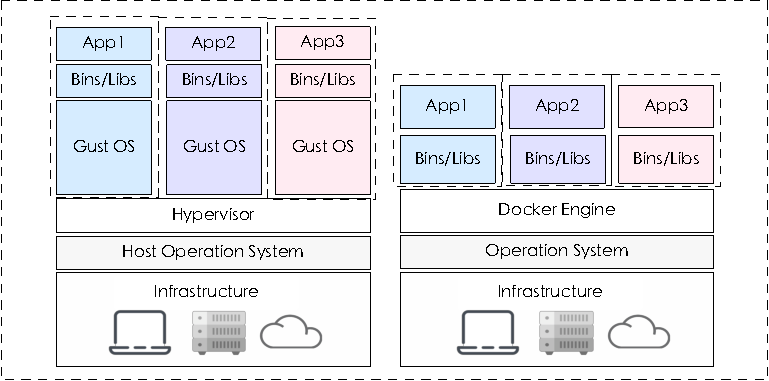
\includegraphics{docker-structure}
	\caption{容器与虚拟机对比~\cite{Barik2017Performance}}
\end{figure}
图1-1中基础设施Infrastructure可以是个人电脑、服务器、云主机等,主机操作系统是运行在基础设施上的系统,主要是Linux的各种版本。虚拟机管理系统(Hypervisor)可以实现在主机操作系统上独立运行多个子操作系统,在子操作系统上安装完应用所需的各种依赖后就可以实现应用资源的隔离。相对于虚拟机,Docker要简便很多,当前所有的Linux版本以及MacOS、Windows都能运行Docker,Docker Engine取代了Hypervisor,负责管理Docker容器并与操作系统通信,各种应用直接打包到镜像文件中,实现容器应用的快速启动和重复应用。

对比Docker和虚拟机的架构~\cite{Barik2017Performance, Felter2007An}发现,Docker直接通过守护进程与操作系统进行通信、容器管理以及资源分配,实现容器与主操作系统的隔离。Docker没有资源开销较大的子操作系统,各容器直接与主操作系统共享资源,其虚拟化开销大幅减少,应用启动时间甚至达到毫秒级。用户可以快速构建、部署和交付应用,并且具有较强的跨平台性。
虽然Docker拥有众多的优势,但其隔离仅仅是在进程层面进行,并不能完全隔离整个运行环境。因此,用户需要根据自己的实际应用场景,在彻底隔离运行环境的需求下选择虚拟机技术,如果仅是应用层面的隔离选择容器技术,如数据库、前端、后端等。

\section{容器云资源调度研究概述}
虚拟机是当前云计算提供服务的主要实现形式,也是云计算的核心技术之一,除虚拟机外,容器在云计算中应用越加广泛,容器云发展迅猛。当前容器虚拟技术以Docker为典型代表,这种既能与宿主机共享资源又能为用户提供隔离的虚拟化方案迅速受到人们关注。容器虚拟化技术只需较小的虚拟化开销就可以实现应用的快速部署、开发、测试、交付以及具有较好的跨平台性。以Docker为基础构建的CaaS(Container as a Service)应运而生~\cite{Kozhirbayev2017A},各大互联网公司都投入巨资进行研发,根据451 Research预测,容器作为一种高速成长型的工具,年增幅高达40\%。容器将作为应用最为广泛的云工具,超过OpenStack、PaaS以及其他相关的产品,该机构在调研了125家应用容器厂商后预测,应用容器将从2016年的7.62亿美元增长到2020的27亿美元。容器的管理和调度市场也在进行快速的组合并购,Apprenda收购Kubernetes支持者Kismatic,思科收购Docker Swarm支持者ContainerX等,这些活动都加速了容器云的快速发展。当前较为出色的容器云有Google Container Engine、SAE、 Cloud Foundry、AWS ECS、Red Hat OpenShift等。

容器云和以虚拟机与基础构建的传统云计算系统一样需要一个性能强大的容器编排管理器进行容器调度、创建、销毁、监控、重启、错误恢复以及服务组合等工作。容器调度器既是容器技术普及的重要推力也是决定集群性能和资源利用率的关键因素~\cite{Application2017},当前有三大主流的容器编排引擎~\cite{Usman2016}: Docker Swarm、Apache Mesos以及Google Kubernetes,其中应用最为广泛的要属轻量开源,性能强大的Kubernetes。在调度算法方面Swarm主要包括Random、Spread和Binpack三种;Mesos更多使用传统的调度算法实现资源分配,如DRF(Dominant Resource Fairness)等;Kubernetes使用两阶段算法选取最大评分节点实现容器调度。几种调度模型和算法各有优缺点,用户可以根据自己的需求选取相应的容器调度框架构建其容器云环境,实现更好的资源分配和调度。本文主要对Kubernetes的调度方式进行研究,在多计算框架容器应用进行大数据处理的场景下提升集群资源利用率和负载均衡,使多计算框架容器应用任务执行时间更短。

\section{面向多计算框架的容器云资源调度研究}
当前,容器云平台的容器编排引擎对容器应用的调度大多使用常规的调度方法,研究也主要针对调度算法进行,容器调度器将计算框架的容器应用分解为不关联的单个容器进行资源分配和任务调度,没有综合考虑计算框架的特性。针对大数据处理场景下容器云如何提升资源利用率和任务执行效率的研究较为分散,往往对单个处理框架进行研究,不存在通用调度方法,也几乎没有针对多计算框架容器应用同时执行任务处理的研究。如Hadoop大数据处理框架用于离线数据批处理,是I/O和网络带宽密集型应用,在进行资源调度时应考虑磁盘I/O和网络带宽的影响,尽可能将容器应用部署到数据存储节点上。Spark大数据处理往往用于处理内存密集型应用,在进行容器应用部署时应尽可能分散部署到内存空闲资源较多的节点上。单个计算框架容器应用在进行大数据处理场景下,其处理框架和处理任务的特性往往对资源需求不同。数据中心在使用计算框架容器应用进行大数据处理时,容器调度器应综合考虑各计算框架的特性和处理任务本身的资源需求特点,不能简单分解为单个不关联容器应用进行资源调度。

容器云中容器编排引擎的调度算法通常是一些常规的调度算法,用于解决单个容器应用的资源调度,并没有专门针对多种计算框架容器应用调度的研究,仅有的部分研究也是对特定的计算框架进行。面向多计算框架的容器云资源调度研究的缺失导致容器云对大数据的处理性能低下,资源利用率不高,任务执行时间过长。为了解决多计算框架容器应用对大数据处理问题,本文提出了新的调度方法,提升容器云资源利用率和负载均衡性,进而缩短任务处理时间。

\section{论文主要工作和结构安排}
\subsection{论文的主要工作}
基于Docker容器虚拟化技术的PasS层OpenShift容器云平台使用Kubernetes进行容器管理和调度,该调度方式通过预选和优选两阶段选取评分最优的节点作为容器调度的目标,在优选阶段仅考虑内存和CPU的影响因素。本文针对其调度方式造成的资源利用率较低和负载不均衡的缺点,在面向多计算框架的容器云平台Paladin上,设计和实现了一个新的调度方案,本文主要工作如下:
 \begin{enumerate}[(1)]
\item 深入研究Kubernetes调度核心技术,针对其调度算法不足,提出了一种基于多维资源空闲率权重的评价函数和调度方法MRWS(Multidimensional Resource Weights Scheduling)。该方法综合考虑物理节点CPU、内存、磁盘、网络带宽空闲率和已部署的容器应用数量等因素影响,使用模糊层次分析法FAHP(Fuzzy Analytic Hierarchy Process)对集群资源自动建模并求解容器应用多维资源权重参数,选取最大评分节点进行容器调度。
\item 针对MRWS调度策略,在容器云仿真平台ContainerCloudSim上进行大规模调度仿真,并与Random、FirstFit、Kubernetes默认调度策略在资源利用率和负载均衡性方面进行对比。
\item 基于开源OpenShift Origin和Paladin Storage构建面向多计算框架的容器云平台Paladin,该平台支持Hadoop、Spark、MPI、Storm等十多种分布式处理框架,用户可以快速构建大数据处理环境和容器伸缩。
\item 在Paladin上设计并实现MRWS调度策略,针对多计算框架下大数据处理场景,比较MRWS与其他调度策略下的集群性能。新的调度策略无论在单计算框架容器应用还是多计算框架容器应用混合执行效率都有极大的提升。
\end{enumerate}

\subsection{本文结构安排}
本文总共分为六个章节,第一章主要阐述传统虚拟机技术构建的云计算和Docker容器技术构建的容器云的区别,云计算底层虚拟化技术和基本架构、云计算服务模式和云计算资源调度方法。接着介绍容器云底层的Docker虚拟化技术,一些典型的容器云产品,容器云中三大主流的容器编排器。针对计算框架容器应用进行大数据处理场景下容器云资源调度器的不足,引出本文需要研究解决的问题。
第二章主要综述容器云资源调度模型,比较分析容器云中典型的集中式调度、两层调度和共享状态三种调度模型,并以Docker Swarm、Mesos和Kubernetes为例阐述三种调度模型的架构和优缺点。最后针对Kubernetes共享状态调度模型容器编排管理器的组织架构、组件、任务处理流程、原理以及其调度的不足进行深入分析。
第三章提出一种全新的综合考虑容器应用和集群物理资源特点的调度方案MRWS,用于解决OpenShift容器云平台下Kubernetes共享状态调度器性能的不足。新方案主要包括调度流程优化、多维资源建模、空闲资源评分,反馈器的设计、权重参数的求解以及负载均衡度评价等。
第四章使用FAHP方法解决新的调度方案中多维资源权重的问题,对容器应用和集群资源进行数学建模、自动构建满足一致性要求的模糊成对比矩阵和判断矩阵,自动求解应用资源权重参数。
第五章首先在ContainerCloudSim容器云仿真平台上进行大规模调度仿真,对比分析MRWS和Kubernetes默认调度方法、FirstFit以及Random调度方法在集群资源利用率、负载均衡度方面的性能。然后在容器云平台Paladin上开发部署十几种分布式计算框架,设计和实现MRWS调度方法,在大数据处理的多计算框架场景下进行性能测试。最后一章对本文工作进行总结,展望未来的研究方向。

